\section{Implementierung}\label{kap_implementierung}

Im Rahmen meiner Projektarbeit im Wintersemester 2014/15 wurde der in \cite{cima_paper} beschriebene Algorithmus in einem Java-Applet von mir implementiert. Ziel war es, den Algorithmus visuell darzustellen und ihn anhand des Applets in einem kurzen Vortrag vorzustellen.
\\
\\
Als Bestandteil dieser Bachelorarbeit wurde das Applet mit der in Kapitel \ref{modifizierterAlgoChapter} beschriebenen Modifikation erweitert, und die in Kapitel \ref{kap_pot} entwickelten Algorithmen in das Applet integriert.


\subsection*{Benutzung des Applets}

Im Folgenden wird kurz beschrieben, wie das Applet benutzt werden kann.

\subsubsection*{Den Baum erstellen und ändern}

Man kann einen Baum (bzw. einen Baumknoten) erstellen, indem mit einem Linksklick in das leere Applet geklickt wird. Sofort erscheint ein Wurzelknoten.\\
Mit einem Linksklick auf einen Knoten fügt man ihm einen Kindknoten hinzu. Mit einem Rechtsklick auf einen Knoten wird dieser zusammen mit dem gesamten Teilbaum gelöscht.\\
Die Kantengewichte lassen sich ebenfalls mit einem Klick verändern. Ein Linksklick erhöht das entsprechende Kantengewicht um 1, ein Rechtsklick reduziert das Kantengewicht um 1. Allerdings können die Kantengewichte nicht kleiner als 1 werden.


\subsubsection*{Verwendung des Applets}

Nachdem man einen Baum erstellt hat, gibt es mehrere Funktionen, die ausgewählt werden können.\\

\begin{itemize}
	\item Man kann die Nachrichtenberechnung sowohl von dem ursprünglichen Algorithmus (Kapitel \ref{kap_algorithmus}), als auch von der Modifikation (Kapitel \ref{modifizierterAlgoChapter}) ausführen. Dazu wählt man in der Kopfzeile im Applet zunächst aus, welcher Algorithmus benutzt werden soll (siehe Abb. \ref{applet_a}). Wird der modifizierte Algorithmus ausgewählt und man möchte diesen ohne Potential berechnen lassen, so gibt man als Potential den Wert 0 ein. Im Anschluss kann mit den verfügbaren Knöpfen in der Fußzeile des Applets ausgewählt werden, ob die Berechnung animiert, oder ob das Ergebnis sofort angezeigt werden soll. Bei der Animation wird immer in der Ecke oben links beschrieben, wie jede einzelne Nachricht zustande kommt. Dazu werden die entsprechenden Elemente des Baumes eingefärbt und mit Hilfe des Textes in Kurzform erklärt, woraus die Berechnung entsteht. Ein Beispiel für eine Erklärung der Nachricht lässt sich in Abb. \ref{applet_b} finden. Nachdem alle Nachrichten verschickt wurden, berechnet jeder Knoten, wie viele Agenten benötigt werden, um den gesamten Baum von diesen Knoten aus zu dekontaminieren. Dieser Wert wird am Ende in jedem Knoten angezeigt. Nach Abschluss des Algorithmus wird einer der Knoten mit minimaler Agentenzahl ausgewählt und als Homebase markiert.
	
	\item Alternativ zur Nachrichtenberechnung kann man sich die beiden Algorithmen aus Kapitel \ref{kap_pot} visuell darstellen lassen. Möchte man den Algorithmus aus Kapitel \ref{kap_pot=1} auswählen, so gibt man im Applet für das Potential den Wert 1 ein. Soll der Algorithmus aus Kapitel \ref{kap_pot>=1} benutzt werden, so muss für das Potential ein Wert größer als 1 eingegeben werden (siehe Abb. \ref{applet_a}). Wurde der gewollte Algorithmus ausgewählt, kann man sich die Nachrichten einzeln animieren lassen, oder auswählen, dass das Ergebnis sofort angezeigt werden soll. Auch hier wird während der Animation erklärt, wie in jedem einzelnen Schritt die erweiterte Nachricht berechnet wird (siehe Abb. \ref{applet_b}), die in dem jeweiligen Algorithmus benutzt wird. \\
	Man muss beachten, dass die Potentialberechnung nur mit der modifizierten Variante des Algorithmus ausführbar ist. Am Ende dieses Algorithmus wird angezeigt, wie viele Agenten jeder Knoten zur Dekontamination benötigt, welcher Knoten die Homebase ist, und, falls möglich, welche Kante reduziert werden sollte, um die Agentenzahl möglichst weit zu reduzieren (siehe Abb. \ref{applet_c}).
	
	\item Außerdem lässt sich im Applet animieren, wie nach erfolgreicher Nachrichtenberechnung die Dekontamination des Baumes funktioniert. Alle bereits dekontaminierten Knoten werden im Applet während der Animation grün eingefärbt, alle kontaminierten Knoten rot. Die Strategie der Agenten ist  monoton. Dies bedeutet, dass jeder Knoten, der schon einmal dekontaminiert wurde, nicht mehr kontaminiert werden kann, da an den entsprechenden Stellen im Baum Wachen aufgestellt werden. Sind alle Knoten dekontaminiert, ist der Algorithmus abgeschlossen. Ein Beispiel hierfür lässt sich in Abbildung \ref{applet_d} finden.
\end{itemize}

Alle Animationen können entweder als Ganzes abgespielt oder in einer Step-by-step-Animation in Teilen durchgeführt werden. \\
In der oberen rechten Ecke des Applets wird beschrieben, welche Information das Applet in den einzelnen Knoten anzeigt. Vor und während der Berechnung steht in allen Knoten das entsprechende Knotengewicht (siehe Abb. \ref{applet_a} und \ref{applet_b}). Nach der Berechnung wird die minimale Anzahl an Agenten angezeigt, die im entsprechenden Knoten benötigt wird, um den gesamten Baum zu dekontaminieren (Abb. \ref{applet_c}). Bei der Dekontamination erscheint im Knoten die Information, wie viele Agenten sich zu dem Zeitpunkt im Knoten befinden (Abb. \ref{applet_d}).\\
Alle Optionen, die im Applet verfügbar sind, werden eingeblendet. Alle in dem Moment nicht verfügbaren Optionen werden ausgeblendet, um eine bessere Übersicht zu gewährleisten.


\begin{figure}[h]
	\subfigure[Verschiedene Einstellungs- und Nutzungsmöglichkeiten, welche das Applet bietet, sobald ein Baum erstellt wurde.
	\label{applet_a}]{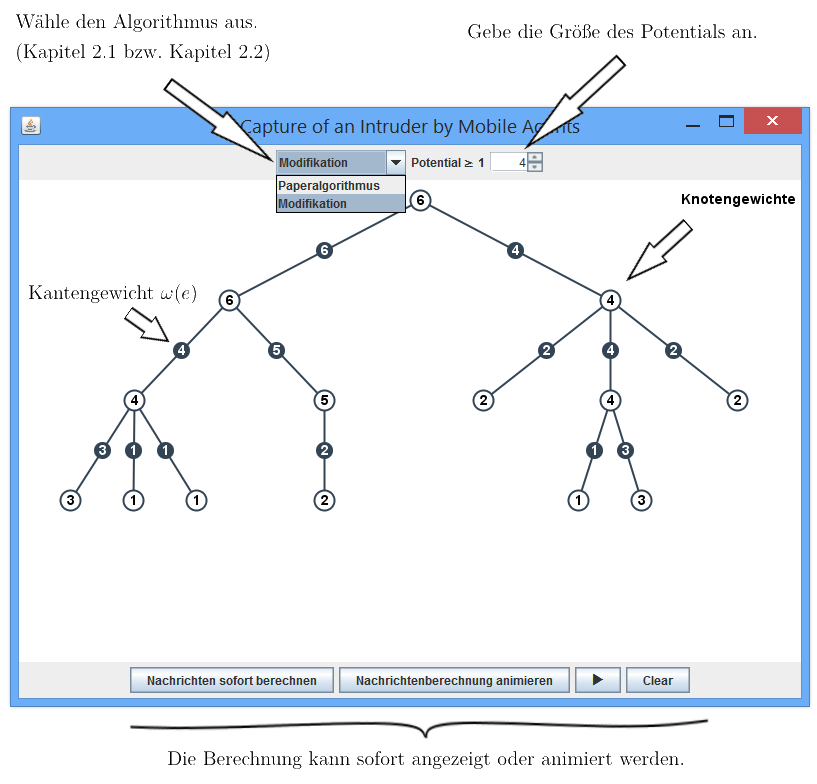
\includegraphics[width=0.84\textwidth]{bilder/abb_erklaerung1.png}}
	%	\hfill  
	%lösche die neue line und füge das \hfill wieder ein um die bilder nebeneiander zu haben
	
	\subfigure[Informationen über die aktuell berechnete Nachricht, bei allen Algorithmusvarianten. Hier: Erweiterte Nachricht aus Kapitel \ref{kap_pot>=1} \label{applet_b}.]{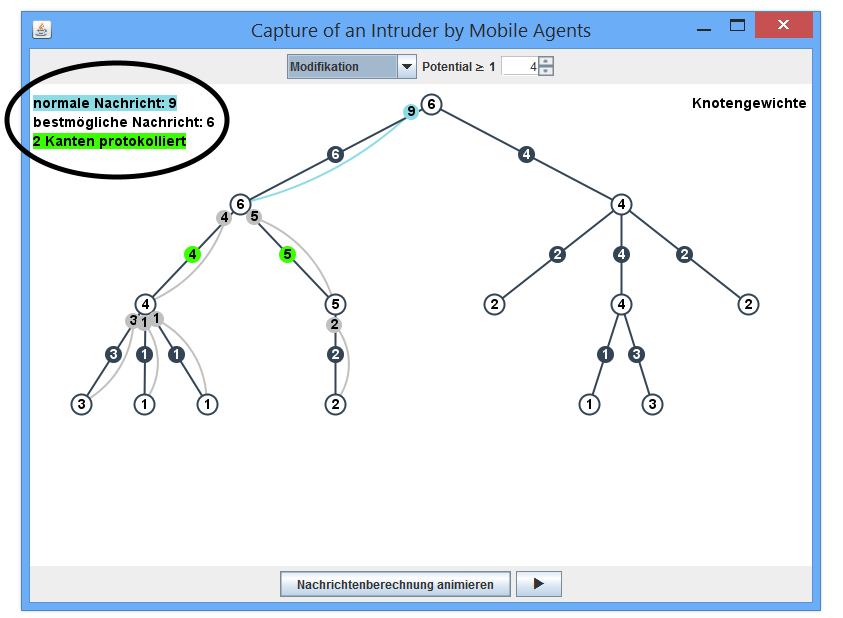
\includegraphics[width=0.84\textwidth]{bilder/abb_erklaerung2.png}} 
	%	\hfill
	
%	\caption{Die Anwendung des Applets wird anhand eines Beispiels verdeutlicht.}
	
\end{figure}
\begin{figure}[h]

%	\ContinuedFloat
	
	\subfigure[Nach der Berechnung wird das Ergebnis, auf welche Kanten das Potential eingesetzt werden kann, angezeigt, indem die entsprechenden Kanten eingefärbt werden. \label{applet_c}]{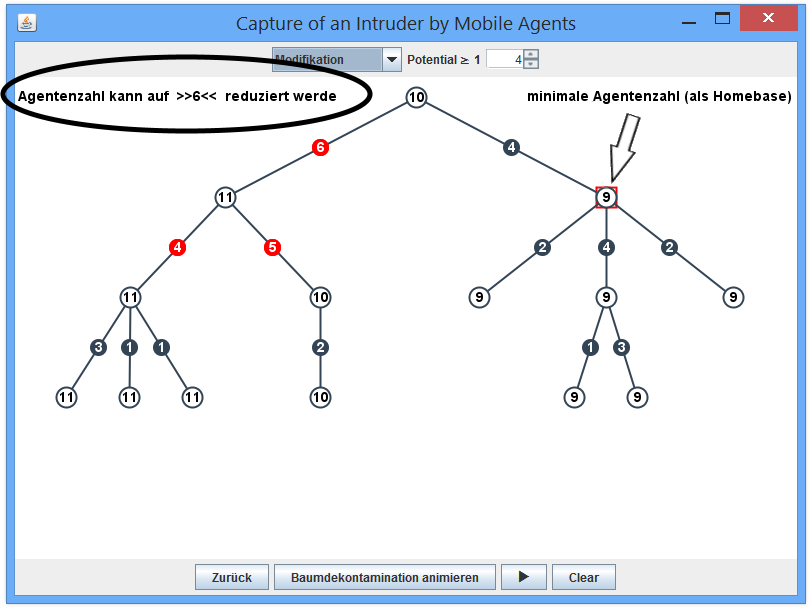
\includegraphics[width=0.84\textwidth]{bilder/abb_erklaerung3.png}}  
	
	\subfigure[Die Agenten dekontaminieren den Baum suzzessive. Dafür müssen an bestimmten Stellen Wachen aufgestellt werden. \label{applet_d}]{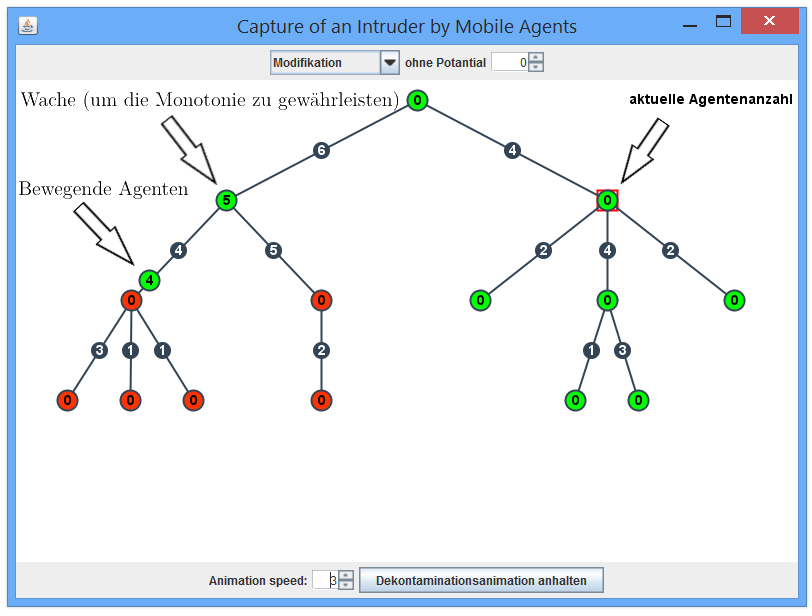
\includegraphics[width=0.84\textwidth]{bilder/abb_erklaerung4.png}}  
	
	\caption{Die Anwendung des Applets wird anhand eines Beispiels verdeutlicht. (Quelle: Eigene Darstellung im Applet)} 
	
\end{figure}	
